\section*{Источники и решения}

\subsubsection*{Любовь в Клептопии}

Эта головоломка приводится в книге Саймона Сингха \cite{singh};
я узнал её от Кэролайн Калдербэнк, дочке пары математиков Ингрид Добеки и Роба Калдербэнка.
В решении Кэролайн, Ян отправляет Марии ящик с кольцом внутри, навесив на него один из своих замков.
По получении Мария навешивает свой собственный замок на ящик и отправляет её назад с обоими замками.
Когда Ян получает ящик, он снимает свой замок и отправляет ящик опять Марии; вуаля!

Это решение не просто игра;
на нём основан обмен ключами шифрования в протоколе Диффи — Хеллмана, историческим прорывом в криптографии.

В зависимости от предположений, возможны и другие решения.
Моё любимое было предложено компанией участников конференции
«Ga\-the\-ring for Gardner VII», включая оригамиста Роберта Лэнга.
Для этого Ян должен найти замок, ключ от которого имеет большое отверстие, или по крайней мере, отверстие, которое может быть достаточно увеличено сверлением, чтобы ключ мог быть нацеплен за дужку другого замка.
Ян использует этот второй замок, с упомянутым ключом на его дужке, чтобы запереть пустой ящичек, которую он отправляет Марии.
По прошествии времени, достаточном для пересылки (или возможно, после электронного подтверждения от Марии), он отправляет кольцо в другом ящике, запертой первым замком.
Когда Мария получает ящик с кольцом, она открывает её ключом, прикреплённым к первому ящичку, и получает кольцо.

\subsubsection*{Черви и вода}

Это скорее инженерная головоломка, чем математическая.
Она пришла ко мне от Балинта Вирага из Массачусетского технологического института.

Лори действительно может защититься от червей свесив с потолка большой навес, выходящий далеко за кровать.
Но навес должен загибаться внутрь под себя по краям, создавая кольцевой жёлоб, заполненный водой.
(Поперечный разрез навеса показан на рис. \ref{pic:chervi}.)

\begin{figure}[h!]
\centering
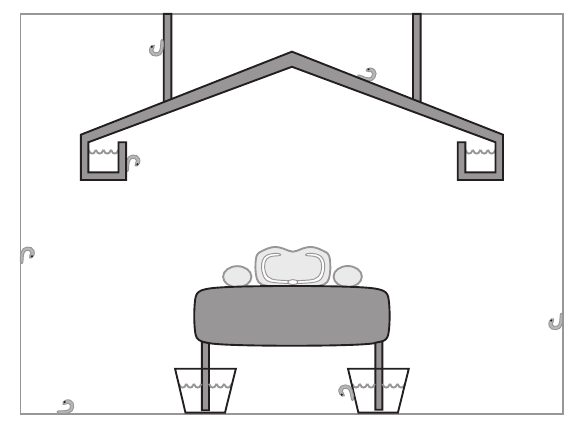
\includegraphics[scale=0.5]{pics/chervi}
\caption{Поперечный разрез Лори в защищённой от червей кровати.}
\label{pic:chervi}
\end{figure}

Если у червей нет способа проникнуть в спальню сверху, то Лори может защититься, обведя комнату по краю жёлобом с водой.

\subsubsection*{Инспекция страусиных яиц}

Вариант этой задачи появился в замечательной книге Джозефа Д. Э. Конхаузера, Дэна Веллемана и Стэна Уэгона \cite{konhauser-velleman-wagon}.

Часто полезно считать данное число (в нашем случае 102) переменной, даже если в конечном счёте нас интересует лишь одно значение.
Пусть $f(k)$ --- максимальное число этажей, которые можно проверить не более чем за $k$ бросков, имея вначале два яйца.
Таким образом, $f(1) = 1$ (прочность яйца может быть $0$ или $1$).
Предположим, что Оскару разрешено сделать $k$ бросков, и он делает первый с $n$-го этажа.
Если яйцо разбилось, то Оскару придётся бросить единственное оставшееся яйцо с 1-го этажа, затем с 2-го и так далее до $(n-1)$-го в худшем случае;
так что $n = k$ это наилучший вариант.
Если яйцо пережило падение с $k$-го этажа, то придётся проверить все этажи выше оставшимися $k-1$ броском (используя два яйца).
Следовательно, $f(k - 1) + k$ это максимальное число этажей, которые можно обработать,
и мы получили рекурсию $f(k) = f(k - 1) + k$.

Прямым вычислением получаем, что $f(2) = 3$, $f(3) = 6$, $f(5) = 10$ и так далее; в общем случае $f(k)$ равно сумме чисел от $1$ до $k$.
Поскольку таких чисел $k$, а их среднее равно $(k + 1)/2$, их сумма (иногда называемая «$k$-ым треугольным числом»), составляет $k(k + 1)/2$.
Первое значение $f(k)$, достигающее 102, это $f(14) = 14 \times 15/2 = 105$, то есть в худшем случае Оскару понадобится $14$ бросков.
Рекурсия указывает и на то как это сделать;
в нашем случае, трёхэтажный запас позволяет Оскару сбросить первое яйцо с одиннадцатого, двенадцатого, тринадцатого или четырнадцатого этажа.
Любой другой вариант может потребовать лишнего броска.

Давайте посмотрим, что происходит с тремя яйцами.
Определим $g(k)$ как максимальное число этажей, которые можно обработать $k$ бросками, начиная с трёх яиц.
Теперь Оскару нужно обработать $g(k \z- 1)$ этажей выше уровня первого броска, если яйцо переживёт падение;
или же $f(k - 1)$ этажей ниже этого уровня (тот же $f$, что и выше), потому что теперь у него лишь два яйца.
Получаем новую рекурсию: $g(k) = g(k-1) + 1 + (k - 1)k/2$, что даёт $g(2) = 3$ (пока без улучшений), но $g(3) = 7$.
В общем случае получаем $g(k)=k(k^2+5)/6$ и наименьшее значение $k$, для которого 
$g(k)\ge 102$, равно $9$.
То есть, если у Оскара есть три яйца,
то ему потребуется максимум девять бросков чтоб обработать Эмпайр-стейт-билдинг.

В общем случае, если $k$ велико, то число этажей, которые можно обработать, имея вначале $m$ яиц, равно $k^m/m!$ плюс члены низших порядков.
Отсюда следует, что с $m$ яйцами и небоскрёбом в $n$ этажей, где  $n$ намного больше $m$, число бросков, необходимых в худшем случае, будет около $(m!\times n)^{1/m}$.

\subsubsection*{Опасная картина}

Эту интересную головоломку предложил Джулио Дженовезе, аспирант в Дартмуте, который узнал её из нескольких источников в Европе.

Один из способов повесить картину изображён на рис. \ref{pic:kartina2}, с зазором, чтобы можно было в нём разобраться.
Шнур проходит над первым гвоздём,
далее идёт петля вокруг второго,
проходит опять над первым гвоздём, и затем снова петля вокруг второго гвоздя, но на этот раз с половинным поворотом.

\begin{figure}[h!]
\centering
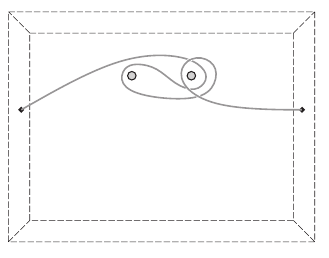
\includegraphics[scale=1]{pics/kartina2}
\caption{Эта картина упадёт если выскочит любой из двух гвоздей.}
\label{pic:kartina2}
\end{figure}

Существуют также некоторые нетопологические решения: например, можно сдавить петлю между двумя близко расположенными гвоздями, предполагая, что ширина головки гвоздя не намного больше толщины шнура.
Но зачем полагаться на трение, когда можно использовать математику?

\begin{addedbytheeditors}
Попробуйте повесить картину на $n$ гвоздей так, чтобы она упала если выскочит любой из них.
А можно ли повесить так, чтоб картина осталась висеть при выпадании одного гвоздя, но падала при выпадании двух?
Хороший обзор подобных задач дан в \cite{demaine2014}, но он не включает результата из \cite{gartside-greenwood}, дающего наилучий способ решения задачи с $n$ гвоздями (без заузливания шнура).
\end{addedbytheeditors}

\subsubsection*{Дефективный кодовый замок}

Этот шедевр комбинаторики достался мне от Амит Чакрабарти из Дартмута;
он был предложен Восточной Германией для Международную математическую олимпиаду 1988 года.

Задачи такого рода лучше решать геометрически.
Пространство всех комбинаций представляет собой комбинаторный куб $8 \times 8 \times 8$.
Каждый раз, когда мы проверяем точку куба, мы вычёркиваем все точки на трёх её координатных линиях.

Представив задачу таким способом, должно быть видно, что лучший способ вычеркнуть все точки это брать все тестовые точки в двух противоположных осьмушках $4 \times 4 \times 4$ нашего куба.
Так можно догадаться до следующего решения.

Давайте проверим все комбинации с числами из $\{1, 2, 3, 4\}$, сумма которых кратна $4$.
Их всего шестнадцать, так как если вы выбираете числа на первых двух (или любых двух) дисках, то число на третьем определяется однозначно.
Теперь попробуем те же комбинации, добавив $(4,4,4)$, то есть, добавив $4$ к каждому из трёх чисел;
их ещё $16$, и мы утверждаем, что вместе эти $32$ комбинации вычёркивают все.

Проверка довольно лёгкая.
Правильная комбинация должна иметь либо два (или более) числа из $\{1, 2, 3, 4\}$, либо два или более числа из  $\{5, 6, 7, 8\}$.
В первом случае существует единственное положение третьего диска (это число в правильной комбинации может не входить в $\{1, 2, 3, 4\}$), так что получена тройка среди первых $16$ тестовых комбинаций.
Второй случай аналогичен.

А вот способ Амита (есть и другие), объясняющий, что нельзя обойтись $31$-й или менее тестовой комбинацией.
Предположим, что $S$ --- это покрытие, и $|S| = 31$.
Пусть $S_i = \{\,(x, y, z) \z\in S : z = i\,\}$ будет $i$-м уровнем $S$.

Рассмотрим три множества:
$A=\{1, 2, 3\}$,
$B = \{4, 5, 6, 7, 8\}$,
и $C \z= \{2, 3, 4, 5, 6, 7, 8\}$.
По крайней мере, один уровень $S$ должен содержать три или меньше точек;
можно считать, что это $S_1$, и $|S_1| = 3$.
(Если $|S_1| \le 2$, то дойти до противоречия ещё проще.)
Точки $S_1$ должны лежать в некотором $3 \times 3 \times 1$ подкубе;
можно считать, что они лежат в $A \times A \times {1}$.

Заметим, что $25$ точек в $B \times B \times \{0\}$ должны быть вычеркнуты точками, не входящими в $S_1$.
Никакие две из них не могут быть вычеркнуты одной точкой в $S$.
Следовательно, $S - S_1$ содержит подмножество $T$ размером $25$, которое лежит в подкубе $B \times B \times C$.
Теперь рассмотрим множество $P = \{\,(x, y, z) : z \in C, (x, y, 1) \notin S_1 , (x, y) \notin B \times B\,\}$.
Легко подсчитать, что $|P| = (64-3-25) \times 7 = 252$.
Точки в $P$ не вычёркиваются $S_1$, и каждая точка в $T$ может вычеркнуть не более $3 + 3 = 6$ точек в $P$. Следовательно, есть по крайней мере $252 - 6 \times 25 = 102$ точки в $P$, которые должны быть вычеркнуты точками в $S - S_1 - T$.

Однако осталось всего $|S - S_1 - T | = 31 - 3 - 25 = 3$ тестовых точек, и каждая из них вычёркивает ровно $22$ точки.
Поскольку $22 \times 3 = 66 \z< 102$, приходим к противоречию. 

\subsubsection*{Альтернативные кубики}

Эта задача настолько известна, что у её решение есть имя: «кубики Шихермана».
В заметке Мартина Гарднера 1978 года \cite{gardner1978} или в ego книге \cite{gardner1989} можно узнать об их открытии полковником Джорджем Шихерманом, сейчас проживающим в Уэйсайд, Нью-Джерси.
Единственная пара кубиков Шихермана имеет метки $\{1, 3, 4, 5, 6, 8\}$ и $\{1, 2, 2, 3, 3, 4\}$.

Возможно, вы нашли ответ перебором, и это вполне подходящий способ решения.
Однако есть и другой способ, иллюстрирующий мощный математический инструмент --- \emph{производящие функции}.

Идея в том, чтоб сопоставить кубику многочлен от переменной $x$, в котором коэффициент при $x^k$ равен числу граней кубика с меткой $k$.
Обычный кубик, например, будет соответствовать многочлену $f(x) = x \z+ x^2 \z+ x^3 \z+ x^4 \z+ x^5 \z+ x^6$.

Ключевое наблюдение заключается в том, что результат броска двух (или более) кубиков представлен произведением их многочленов.
Например, если мы бросаем два обычных кубика, то коэффициент $x^{10}$ в произведении (то есть в $f(x)^2$) есть число способов выбора двух членов из $f(x)$, произведение которых равно $x^{10}$ ---
это $x^4 \times x^6$, $x^5 \times x^5$ и $x^6 \times x^4$; они представляют три способа получить сумму $10$.

Следовательно, если $g(x)$ и $h(x)$ --- многочлены наших кубиков, то $g(x) \times h(x) = f(x)^2$.
Многочлены, как и числа, единственным способом разлагаются на простые сомножители;
многочлен $f(x)$ разлагается как $x(x + 1)(x^2 + x + 1)(x^2 - x + 1)$.
Чтобы получить произведение $g(x)$ и $h(x)$ равное $f(x)^2$, нам нужно взять каждый из этих $4$ сомножителей и добавить по одной его копии в $g(x)$ и в $h(x)$, или же две его копии в один либо в другой.
Но есть следующие ограничения:
в полученных многочленах $g(x)$ и $h(x)$ не может быть свободных членов (это бы означало, что некоторые стороны помечены нулём);
не допускаются отрицательные коэффициенты;
также сумма коэффициентов в каждом из этих многочленов должна равняться 6.


Единственный решение (кроме $g(x) = h(x) = f(x)$) это
\[g(x)
=
x(x + 1)(x^2 + x + 1)
=
x + 2x^2 + 2x^3 + x^4\]
и
\[h(x)
=
x(x + 1)(x^2 + x + 1)(x^2 - x + 1)^2
=
x + x^3 + x^4 + x^5 + x^6 + x^8,\]
или наоборот.

Мы всё ещё использовали перебор, но таким методом можно решать задачи посложнее.
Во-первых, можно придумать альтернативы для пары восьмигранных игральных костей, пронумерованных от $1$ до $8$ (есть три альтернативных варианта), или для бросания трёх обычных кубиков (много способов).

Читателям, которые хотят поглубже изучить эту тему, стоит обратиться к отличной статье Джо Галлиана и Дейва Русина \cite{gallian-rusin}.

\subsubsection*{Совпадение монет}

Эту задачу предложил мне Одед Регев, из Техниона, в Израиле.
Сонни и Шер могут выиграть более чем в 2/3 случаев.
Для этого разделим последовательность бросков на блоки по три.
Перед каждым блоком Шер \emph{оповещает} Сонни, будут ли в следующем блоке в основном орлы или решки;
если первое, Сонни говорит «ООО» в этом блоке; если второе, то «РРР».

Но как Шер передать эту информацию?
Чаще всего Сонни ошибается (в точности) раз в блоке.
Перед этим броском Шер говорит «О», сообщая, что в следующем блоке будут в основном орлы, и «Р» в противном случае.
Для двух других бросков в текущей тройке Шер даёт правильный ответ (вместе с Сонни), гарантируя две из трёх побед.
Если случится, что Сонни может угадать все три броска в текущей тройке,
то один раз --- скажем на последнем броске, Шер действует, как описано выше, даже если это стоит им потери одной победы.
Таким образом, после первого блока Сонни и Шер будут набирать две победы из трёх, когда блок состоит из двух орлов и одной решки или двух решек и одного орла.
Когда блок состоит полностью из орлов или полностью из решек (что происходит с вероятностью 1/4), они получают две победы из трёх в половине случаев и три из трёх в остальной половине.
Значит доля успеха составит $3/4 \times 2/3 + 1/4 \times 5/6 = 17/24 > 70.8\%$.
Обратите внимание, что даже в наихудшем случае (например, если последовательные орлы и решки выбираются противником, а не случайны) этот метод гарантирует долю успеха хотя бы $2/3$.

Оливье Госснер, Пенелопа Эрнандес и Абрахам Нейман \cite{gossner} доказали, что с более сложными версиями этой схемы Сонни и Шер могут приблизиться к любой доле успеха равной $x$, где $x$ --- единственное решение уравнения
\[-x \log_2 x - (1 - x) \log_2 (1 - x) + (1 - x) \log_2 3 = 1,\]
и лучшего добиться нельзя.
Более того, это утверждение остаётся верным независимо от того, случайны ли броски монеты или нет!
Поскольку это значение $x$ составляет около $0{,}8016$, Сонни и Шер могут на самом деле добиться победы более чем в $80\%$ случаев, даже когда оппонент играет против них.

\subsubsection*{Имена в ящиках}

У этой головоломки короткая, но увлекательная история.
Она придумана датским специалистом по информатике Петером Бро Милтерсеном;
её версия появилась в завоевавший широкое признание статье, написанной им и Анной Галь \cite{gal-miltersen}.
Однако Милтерсен не знал  решения, пока его коллега Свен Скиум не указал ему на это во время обеда.
В конечном итоге головоломка дошла до меня (в несколько усложнённой форме) через Дорит Ахаронов.

Чтобы её решить, заключённые должны сначала договориться о случайном соответствии ящиков со своими именами.
(Это сделает невозможным разложить имена в ящиках так, чтобы помешать протоколу, описанному ниже.)
Попадая в комнату, каждый заключённый проверяет свой собственный ящик (то есть ящик, с которому соответствует его имя).
Затем он заглядывает в ящик, соответствующий имени, которое он только что нашёл,
затем в ящик, соответствующий имени, найденному во втором ящике, и так далее, пока он не найдёт своё собственное имя или не откроет 50 ящиков.

Вот такая стратегия, но почему она работает?
Соответствие, между именем владельца ящика и именем, найденном в его ящике, представляет собой перестановку из 100 имён, выбранную равномерно случайным образом из набора всех таких перестановок.
Каждый заключённый идёт по циклу перестановки, начиная со своего имени.
Если цикл не длиннее 50, то он находит своё имя.
Если перестановка не длинней 50, то это сработает для всех, и заключённые будут спасены.

Вероятность того, что равномерно случайная перестановка чисел от $1$ до $2n$ не содержит ни одного цикла длиной более $n$, равна по крайней мере, $1$ минус натуральный логарифм от $2$, что составляет около $30,6853\%$.

Чтобы увидеть это, положим $n < k \le 2n$ и сосчитаем перестановки, имеющие цикл $C$ длиной ровно $k$.
Есть $\binom{2n}k$ способов выбрать имена в этом цикле, $(k - 1)!$ способов упорядочить их в $C$
и $(2n - k)!$ вариантов перестановки остальных имён;
произведение этих чисел равно $(2n)!/k$.
Поскольку в данной перестановке может существовать не более одного $k$-цикла, вероятность того, что такой существует, точно равна $1/k$.
Значит вероятность отсутствия длинного цикла равна
\[1-\frac{1}{n}-\frac{1}{n+1}-\dots-\frac{1}{2n}=1-H_{2n}-H_n\]
где $H_m$ --- сумма обратных чисел первых $m$ положительных целых чисел, что приблизительно равно $\ln m$.
Таким образом, наша вероятность будет близка к $1 - \ln 2n + \ln n = 1 - \ln 2$, на самом деле всегда чуть больше этого значения.
Для $n = 50$ мы получаем, что заключённые выживают с вероятностью $31,1827821\%$.
Недавно Юджин  Кертин и Макс Варшауэр \cite{curtin-warshaue} показали, что это решение нельзя улучшить.

Ламберт Брайт и Рори Ларсон, а также независимо Ричард Стэнли из Массачусетского технологического института, предложили следующую вариацию.
Предположим, что каждый заключённый должен заглянуть в \emph{не менее} чем 50 ящиков, и требование для выживания заключается в том, чтобы каждый заключённый \emph{не} нашёл собственное имя?
Несмотря на то, что цель полностью противоположна, похоже, что у заключённых нету лучшего варианта чем как следовать точно той же стратегии.
Однако теперь они выживают лишь, если каждый цикл длиннее $50$, а это происходит только при наличии единственного большого цикла длины $100$ --- шансы составляют ровно $1$ к $100$.
Не очень обнадёживает, но всё же лучше, чем $1$ к $2^{100}$.

Заметим, что у заключённых будут те же шансы, если каждому потребуется заглянуть в $99$ ящиков --- снова они следуют стратегии и выигрывают, когда случайная перестановка является циклом.
В этом случае сразу очевидно, что лучшей стратегии нет.
Ведь самый первый заключённый, чтобы он не делал, выживет с вероятностью $1\%$.
Забавно, что, если следовать этой стратегии, то как только повезло первому заключённому, так автоматически везёт всем остальным!
